\section{Demodulación AM}
Recordando el demodulador en la sección 1.4.2, este se puede aplicar para este contexto, y en particular cabe resaltar la constante $\tau = RC$ para la construcción del demodulador. Como el tono puro tiene 5KHz y la portadora, que tiene 760KHz. Ahora, como $\frac{1}{f_m}>\tau>\frac{1}{f_c} \longleftrightarrow \frac{1}{5000}>\tau > \frac{1}{760000}$, por lo que $\tau$ queda acotado, y en particular, se escoge $\tau = 33ns$ donde $R = 100k\Omega$ y $C = 330pF$. Se escogieron estos valores, pues un capacitor muy bajo no alcanza a demodular, y una resistencia menor haría que la corriente no pase por el capacitor, afectando el resultado. La salida de este demodulador entrega:

\begin{figure}[ht!]
    \centering
    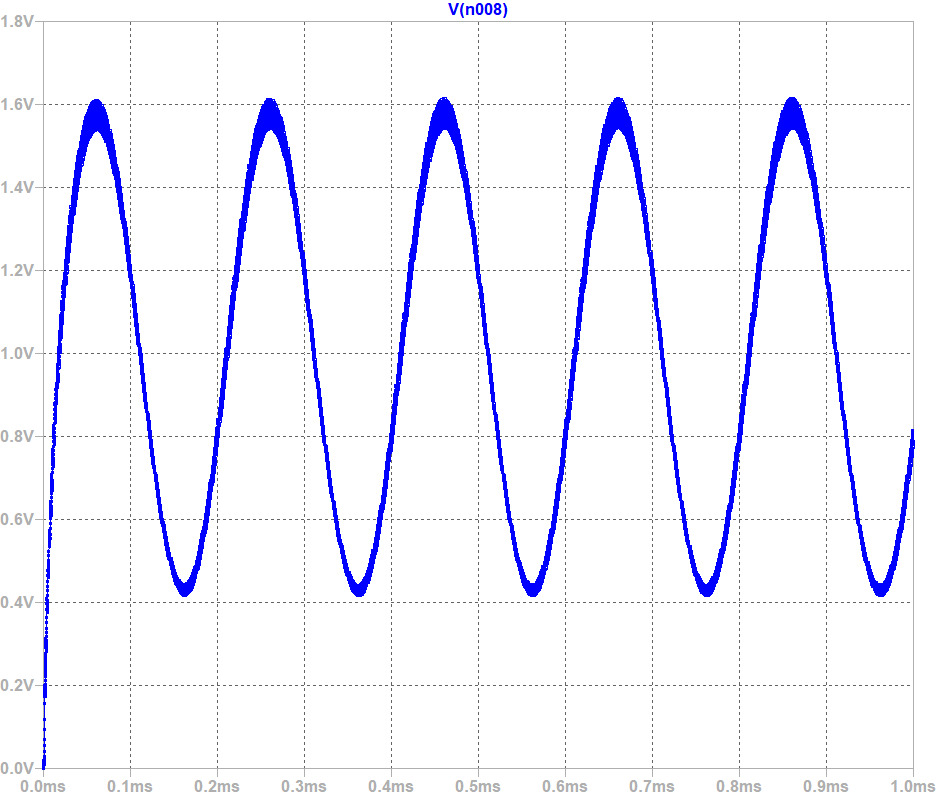
\includegraphics[width=0.75\linewidth]{img/Salida demodulador.jpg}
    \caption{Salida del demodulador}
    \label{fig:demod_output}
\end{figure}

Luego, los requerimientos exigen que la amplitud pk-pk sea de a lo más 1 y que esté centrada en 0, así, viendo que la amplitud pk-pk resultante es de aproximadamente 1.2V, hay que atenuar la señal, cosa que se puede hacer con una configuración inversora con constante $\frac{R2}{R1}=\frac{1}{1.2}$. En particular, no queremos que incluir este bloque afecte la demodulación, es por esto que su impedancia de entrada debe ser alta, es por esto que es preferible una impedancia de 2.4M$\Omega$ y 2M$\Omega$. Por último, hay que deshacerse del offset que tiene la señal, por lo que forzando un voltaje en el nodo - de 0.46V se cumple que la señal esté centrada en 0.Así, la señal de salida es:

\begin{figure}[ht!]
    \centering
    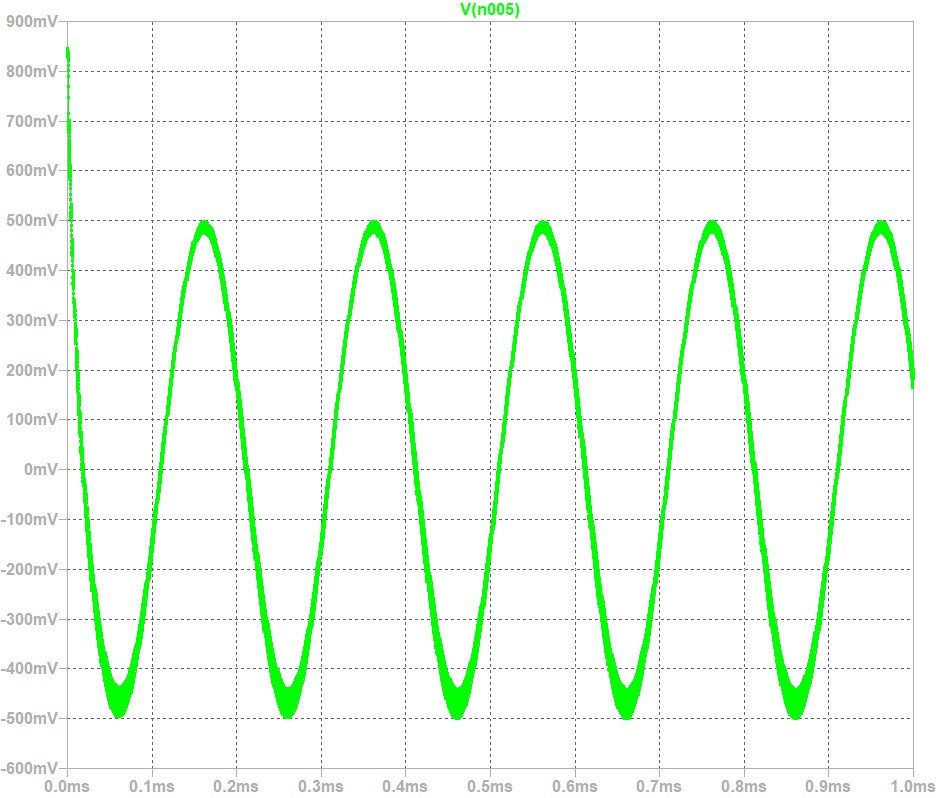
\includegraphics[width=0.75\linewidth]{img/Salida final.jpg}
    \caption{Salida final}
    \label{fig:demod_final}
\end{figure}

Por último, el circuíto propuesto es:

\begin{figure}[htbp]
    \centering
    \begin{circuitikz}[american]

        \draw (0,0) node[left]{$V_{AM}$}
        to[short, o-] (1,0)
        to[D, l=1N4148] (2,0)
        to[short] (3,0) coordinate (nodo1);

        \draw (2.5,0) to[R, l=100k$\Omega$] ++(0,-2) node[ground]{};

        \draw (nodo1) to[short] ++(1.5,0) coordinate (nodo2);
        \draw (nodo2) to[C, l=330pF] ++(0,-2) node[ground]{};

        \draw (nodo2) to[R, l=2.3M$\Omega$] ++(2,0) coordinate (inv_in);

        \draw (inv_in) to[short] ++(0.5,0) node[op amp, anchor=-] (U8) {};

        \draw (U8.out) to[short, -o] ++(1,0) node[right]{$V_o$};

        \draw (U8.out) to[R, l=1M$\Omega$] ++(0,2)-| (inv_in);

        \draw (U8.+) to[short] ++(0,-1) coordinate (plusnode) node[below]{$0.45V$};
    \end{circuitikz}
    \caption{Circuito Demodulador}
\end{figure}
